\documentclass{report}
\usepackage[utf8]{inputenc}
\linespread{1.25}
\usepackage[italian]{babel}
\usepackage[svgnames]{xcolor}
\usepackage{float}

\usepackage[section]{placeins}

\usepackage{listings} %code highlighter
\usepackage{color} %use color
\definecolor{mygreen}{rgb}{0,0.6,0}
\definecolor{mygray}{rgb}{0.5,0.5,0.5}
\definecolor{mymauve}{rgb}{0.58,0,0.82}

\lstset{ %
backgroundcolor=\color{white}, % choose the background color; you must add \usepackage{color} or \usepackage{xcolor}
basicstyle=\footnotesize, % the size of the fonts that are used for the code
breakatwhitespace=false, % sets if automatic breaks should only happen at whitespace
breaklines=true, % sets automatic line breaking
captionpos=b, % sets the caption-position to bottom
commentstyle=\color{mygreen}, % comment style
deletekeywords={...}, % if you want to delete keywords from the given language
escapeinside={\%*}{*)}, % if you want to add LaTeX within your code
extendedchars=true, % lets you use non-ASCII characters; for 8-bits encodings only, does not work with UTF-8
frame=single, % adds a frame around the code
keepspaces=true, % keeps spaces in text, useful for keeping indentation of code (possibly needs columns=flexible)
keywordstyle=\color{blue}, % keyword style
% language=Octave, % the language of the code
morekeywords={*,...}, % if you want to add more keywords to the set
numbers=left, % where to put the line-numbers; possible values are (none, left, right)
numbersep=5pt, % how far the line-numbers are from the code
numberstyle=\tiny\color{mygray}, % the style that is used for the line-numbers
rulecolor=\color{black}, % if not set, the frame-color may be changed on line-breaks within not-black text (e.g. comments (green here))
showspaces=false, % show spaces everywhere adding particular underscores; it overrides 'showstringspaces'
showstringspaces=false, % underline spaces within strings only
showtabs=false, % show tabs within strings adding particular underscores
stepnumber=1, % the step between two line-numbers. If it's 1, each line will be numbered
stringstyle=\color{mymauve}, % string literal style
tabsize=2, % sets default tabsize to 2 spaces
title=\lstname % show the filename of files included with \lstinputlisting; also try caption instead of title
}
%END of listing package%
 
\definecolor{darkgray}{rgb}{.4,.4,.4}
\definecolor{purple}{rgb}{0.65, 0.12, 0.82}
 
%define Javascript language
\lstdefinelanguage{JavaScript}{
keywords={typeof, new, true, false, catch, function, return, null, catch, switch, var, if, in, while, do, else, case, break},
keywordstyle=\color{blue}\bfseries,
ndkeywords={class, export, boolean, throw, implements, import, this},
ndkeywordstyle=\color{darkgray}\bfseries,
identifierstyle=\color{black},
sensitive=false,
comment=[l]{//},
morecomment=[s]{/*}{*/},
commentstyle=\color{purple}\ttfamily,
stringstyle=\color{red}\ttfamily,
morestring=[b]',
morestring=[b]"
}
 
\lstset{
language=JavaScript,
extendedchars=true,
basicstyle=\footnotesize\ttfamily,
showstringspaces=false,
showspaces=false,
numbers=left,
numberstyle=\footnotesize,
numbersep=9pt,
tabsize=2,
breaklines=true,
showtabs=false,
captionpos=b
}

\title{
    TrackER Project \\
    \large Applicazioni e Servizi Web
}

\author{
  Emanuele Dall'Ara - 0001061501\\
  \texttt{emanuele.dallara@studio.unibo.it}
  \and
  Nicholas Ricci - 0001036866\\
  \texttt{nicholas.ricci@studio.unibo.it}}
\date{12 Settembre 2022}

\usepackage{natbib}
\usepackage{graphicx}

\begin{document}
\maketitle
\tableofcontents
\maketitle
\chapter{Introduzione}
\section{Contesto di riferimento}

Il progetto nasce come una soluzione software web-based di \textbf{gestione, tracciamento e vendita dell’energia} sia dal punto di vista dei venditori (\textbf{Vendor}) sia per gli utenti consumatori (\textbf{Buildings Owner}). 

L’obiettivo primario è quello di consentire a ciascun utente di poter visionare e gestire i propri edifici per quanto riguarda la loro produzione (tramite fonti rinnovabili) ed il loro consumo di risorse energetiche.
\par La web application si compone di due principali interfacce: una relativa al Vendor ed una al Buildings Owner raggiungibili soltanto una volta dopo essersi registrati nel sistema.


 
\chapter{Requisiti}
\section{Requisiti Utente}
\par Di seguito sono elencate le principali funzionalità per ogni tipo di account:
\begin{itemize}
  \item \textbf{Vendor}:
  \begin{itemize}
   \item Creare un'organizzazione selezionando il tipo di energie che mette a disposizione dei consumatori;
         \item  Controllare la mole di dati energetici prodotta e consumata; 
         \item Modificare alcune informazioni relative all'organizzazione;
         \item  Controllare i guadagni (totali e relativi ai singoli edifici); 
         \item  Controllare i costi di produzione e delle imposte (totali e relativi ai singoli edifici);
         \item  Controllare lo stato di produzione dei dispositivi installati;
         \item  Personalizzare il proprio account.            
 \end{itemize}
 \item \textbf{Buildings Owner}: 
   \begin{itemize}
   \item Aggiungere i propri edifici sulla piattaforma;
   \item Modificare alcune informazioni dei propri edifici registrati;
      \item Selezionare il contratto di fornitura d'energia che si vuole sottoscrivere per ciascun edificio;
      \item  Monitorare i consumi dei propri edifici;  
         \item  Installare dispositivi di energie rinnovabili;
         \item  Visualizzare la mole di energia prodotta da fonti rinnovabili e il corrispondente guadagno;
         \item Personalizzare il proprio account.            
 \end{itemize}
 \end{itemize}
 
\section{Requisiti Funzionali}
\begin{itemize}
\item Registrazione di un nuovo utente;
\item  Generazione di notifiche e/o avvisi sullo stato dei dati.
\end{itemize}

\section{Requisiti Non Funzionali}
\begin{itemize}
\item Rendere il sistema facile ed intuitivo;
\item Rendere il sistema sicuro mediante meccanismi di autenticazione, autorizzazione e con l'ausilio della crittografia; 
\item Rendere il sistema reattivo;
\item  Rendere il sistema responsive.
\end{itemize}

\chapter{Design}

Il modello utilizzato è di tipo iterativo e basato su User Centered Design con utenti virtualizzati. 
Sono stati individuati gli utenti target dell’applicazione e su di essi si sono sviluppate le Personas che hanno contribuito a sviluppare e comprendere le funzionalità del sistema e i relativi requisiti utente.
Il team ha gestito tutto il progetto tramite \textbf{Issue} su \textbf{GitHub}. Ogni issue aveva un certo grado di priorità permettendo così di organizzare lo sviluppo in vari sprint.
Quindi si è seguito un approccio simile a quello \textbf{AGILE} che ha permesso, in modo incrementale, lo sviluppo delle varie funzionalità in base alla priorità.
Nello svolgimento del progetto e del design delle interfacce si è cercato di rispettare il principio di \textbf{KISS} per risolvere le funzionalità nel modo più semplice possibile. 
Nello sviluppo delle interfacce si è sempre tenuto in considerazione la riusabilità di esse.
Nello sviluppare l'applicazione sono state utilizzate tecnica di Responsive Design, in modo che le pagine web adattino automaticamente il layout per
fornire una visualizzazione ottimale in funzione dell'ambiente nei quali vengono visualizzati: pc, tablet, smartphone sono i principali.
\section{Mockup}
Per la realizzazione dei mockup si è preferito svolgere disegni a penna su carta delle interfacce principali. Questi rappresentano una versione semplificata del prodotto finale.



\subsection{Sign In/Up page}
\begin{figure}[H]
  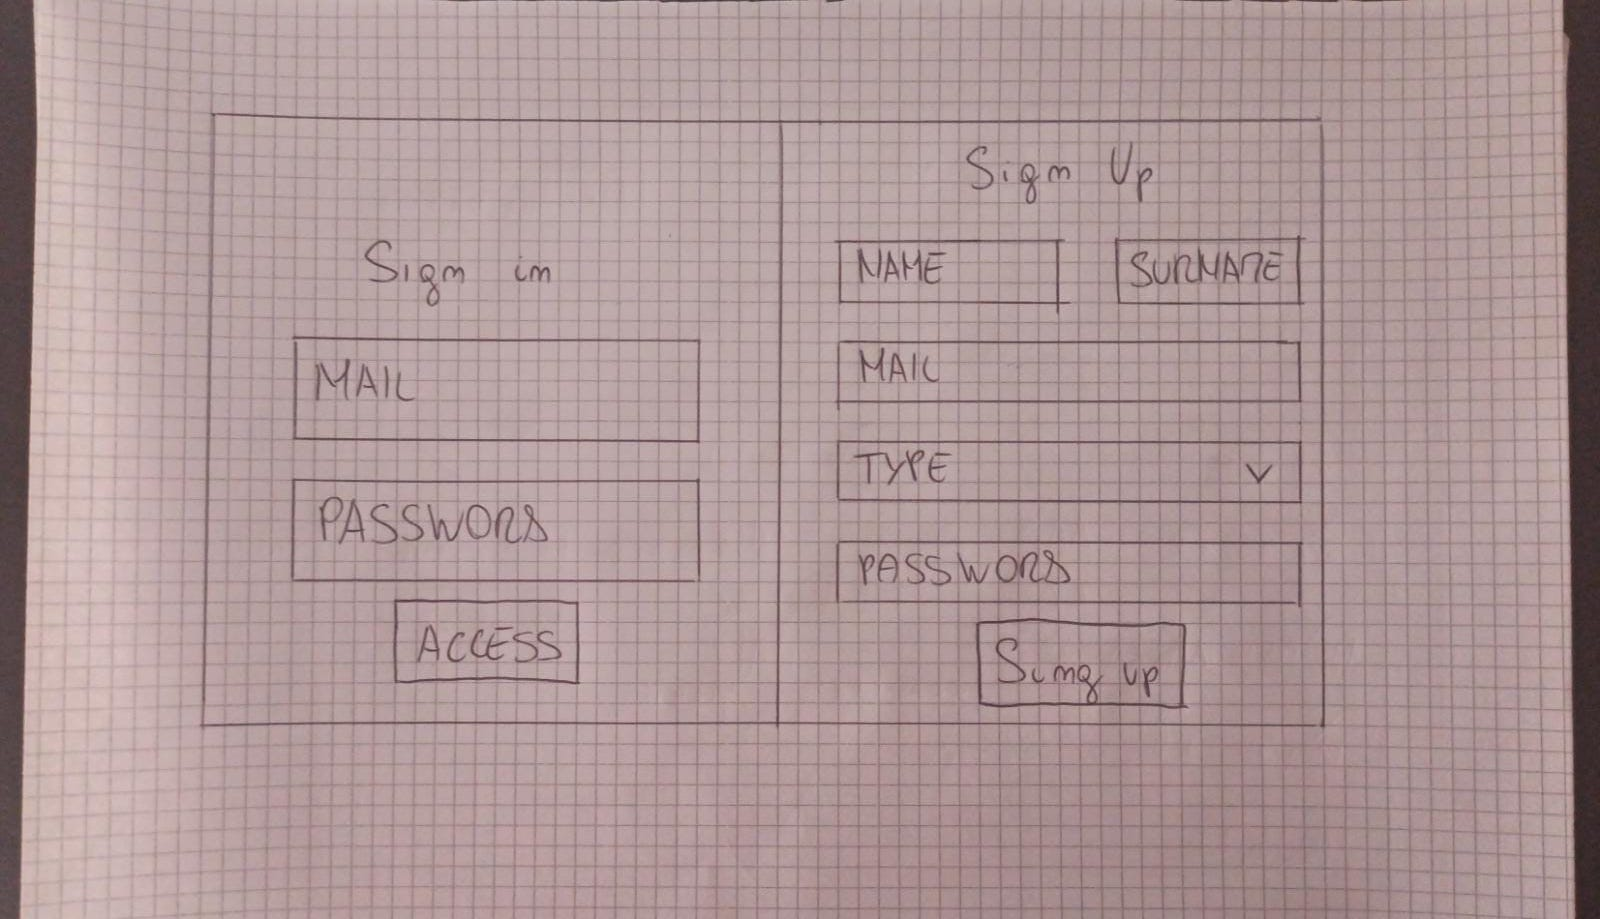
\includegraphics[width=\linewidth]{Sign.jpeg}
  \caption{Sign In/Up page.}
  \label{fig:Sign In/Up page}
\end{figure}
\par Per la form di Sign In/Up all'applicazione si è pensato di suddividere l'accesso e la registrazione all'applicazione in una singola schermata per non disperdere l'utente nelle varie pagine del sistema. La registrazione richiederà il tipo di utente che si vuole creare (Vendor o Buildings Owner) mentre per accedere al sistema sarà necessario effettuare il Sign In  tramite Mail e Password.
\subsection{Account page}
\begin{figure}[H]
  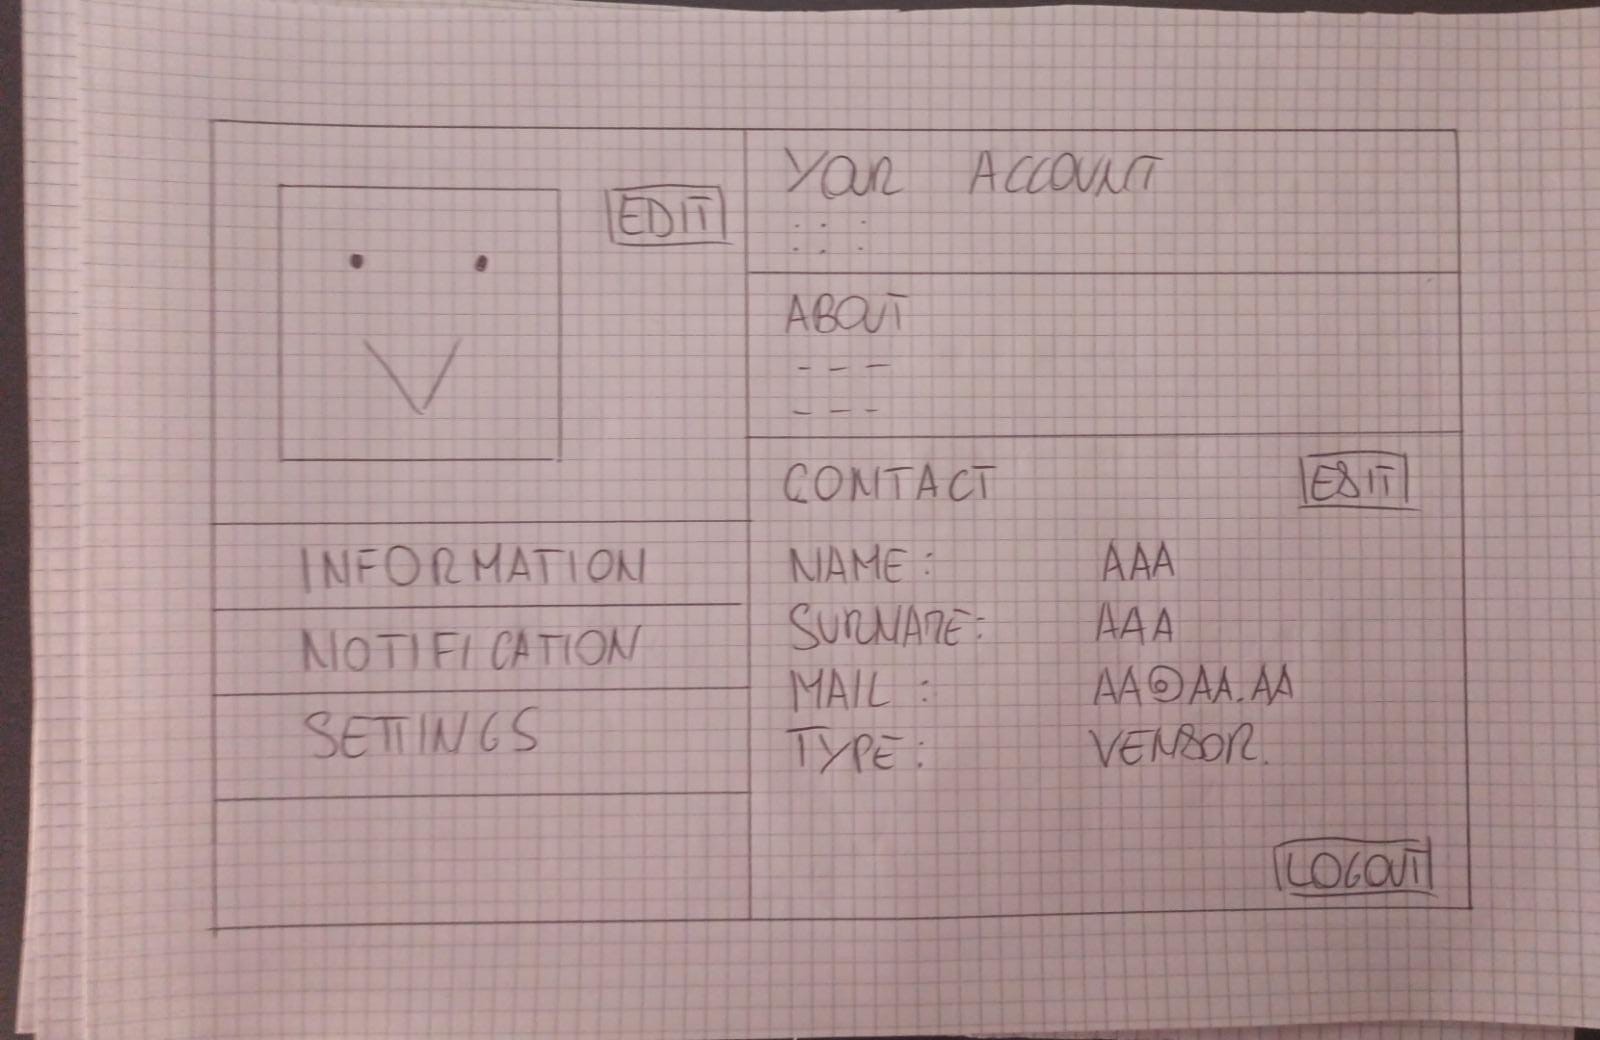
\includegraphics[width=\linewidth]{Account.jpeg}
  \caption{Account page.}
  \label{fig:Account page}
\end{figure}
\par Per la pagina Account si è pensato di creare due sezioni: 
\begin{itemize}
\item una con un menù di navigazione sulle varie iterazioni che l'utente può fare con il suo account(parte sinistra di figura 3.2);
\item una inerente alla renderizzazione dei dati provenienti dalla sezione precedente (parte destra di figura 3.2)
\end{itemize}
La differenza sostanziale tra le due tipologie di account per questa pagina sarà inerente alla personalizzazione dell'avatar in cui, un Vendor, potrà caricare il logo della sua organizzazione mentre un Buildings Owner potrà selezionare un avatar presente nel sistema.
\subsection{Vendor Dashboard}
\begin{figure}[H]
  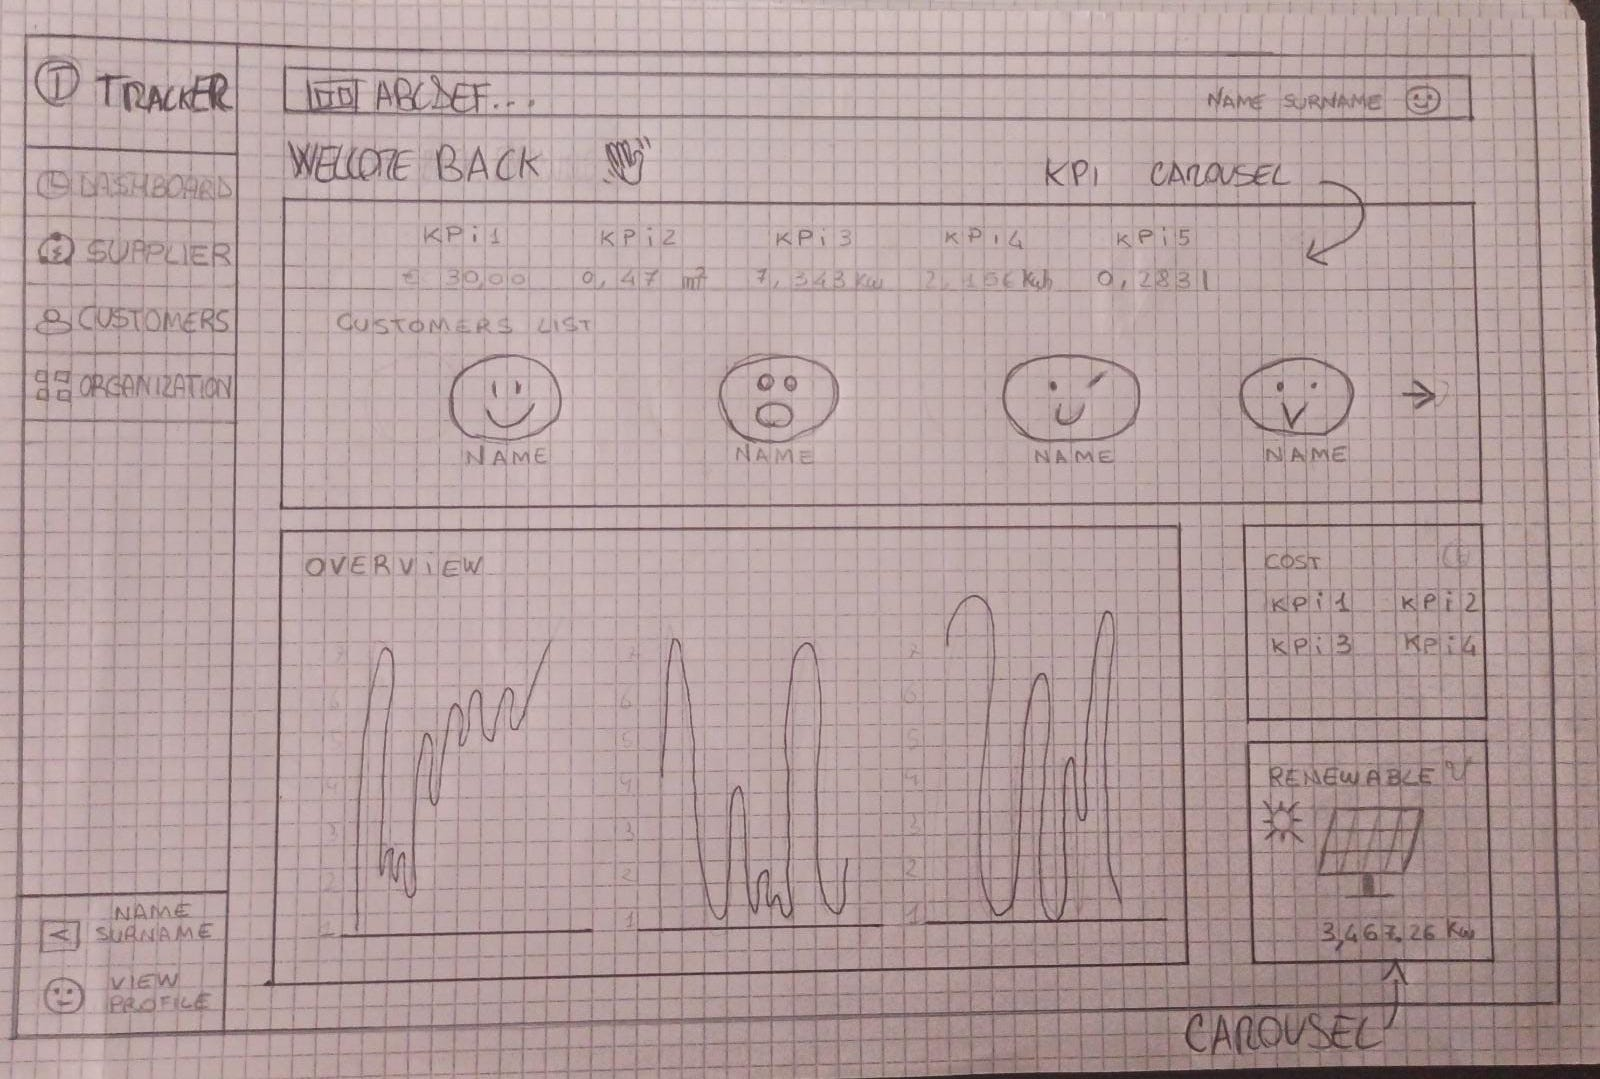
\includegraphics[width=\linewidth]{Vendor.jpeg}
  \caption{Vendor Dashboard.}
  \label{fig:Vendor Dashboard}
\end{figure}
La  Vendor DashBoard avrà come obiettivo principale quello di dare una visione generale sui costi e guadagni di un Vendor.
Questa pagina sarà composta da grafici inerenti ai consumi utente, un collegamento veloce agli edifici utente e una vasta gamma di KPI. 
\FloatBarrier


\subsection{Buildings Owner Dashboard}
\begin{figure}[H]
  \includegraphics[width=\linewidth]{buildingsOwner.jpeg}
  \caption{Buildings Owner Dashboard.}
  \label{fig:Buildings Owner Dashboard}
\end{figure}

La Buildings Owner DashBoard sarà molto simile alla Vendor DashBoard ma il suo obiettivo principale sarà quello di dare una visione generale sui consumi e risparmi energetici di un Buildings Owner.
Questa pagina avrà meno KPI rispetto a quella vendor ma conterrà più grafici inerenti ai consumi. 
\FloatBarrier


\subsection{Buildings page}
\begin{figure}[H]
  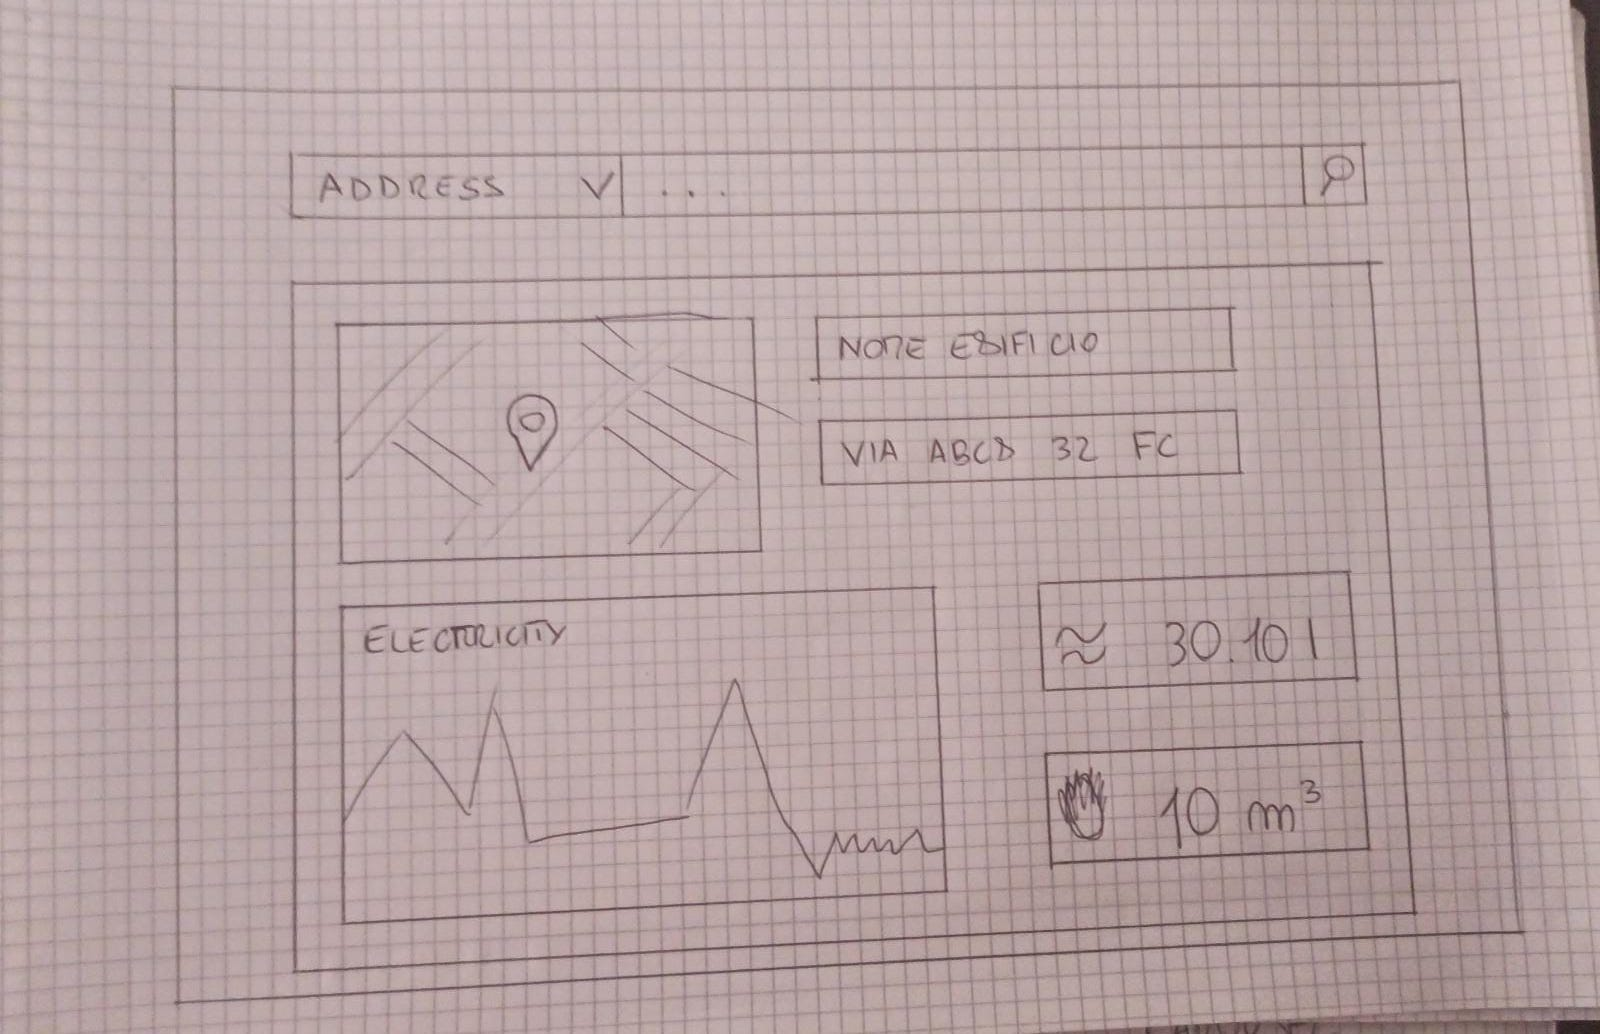
\includegraphics[width=\linewidth]{Buildings.jpeg}
  \caption{Buildings page.}
  \label{fig:Buildings page}
\end{figure}
La Buildings Page sarà composta da più interfacce che rappresentano un singolo edificio. Ogni edifico mostrerà la propria ubicazione tramite una mappa, le sue informazioni principali e i suoi costi totali. 
Si permetterà inoltre ad un utente di poter cercare i propri edifici tramite \textbf{nome edificio} e \textbf{indirizzo edificio}.
\FloatBarrier


\section{Analisi target user}
Sono state costruite diverse Personas sui profili definiti in precedenza (Vendors e Buildings Owners):
\begin{itemize}
 \item \textbf{Personas Gavin}: 
\\ E' il proprietario di Energy Cop (che fornisce energia elettrica, gas e acqua) e vuole monitorare il numero di clienti affiliati e i suoi costi e guadagni totali.
\begin{enumerate}
\item Si registra ed accede alla piattaforma come Vendor;
\item Registra la sua organizzazione come fornitrice di energia elettrica, di gas e di acqua;
\item Accede all'applicazione e verifica i propri costi e guadagni totali.
\end{enumerate}

 \item \textbf{Personas Tony}: 
\\ Possiede un'impresa che fornisce dispositivi di energie rinnovabili (pannelli solari e fotovoltaici) ed ha bisogno di espandere la rete dei suoi clienti.
\begin{enumerate}
\item Si registra ed accede alla piattaforma come Vendor;
\item Registra la sua organizzazione come fornitrice di sole energie rinnovabili;
\item Aggiunge i dispositivi che vende all'interno dell'applicazione;
\item Accede all'applicazione e verifica il numero di clienti totali.
\end{enumerate}

\item \textbf{Personas Francesco}
\\ Possiede una vasta rete di edifici aziendali e vuole verificare i consumi dei propri edifici e possibilmente installare qualche dispositivo di energia rinnovabile per ridurre le spese totali.
\begin{enumerate}
\item Si registra ed accede alla piattaforma come Buildings Owner;
\item Registra i propri edifici sotto un'organizzazione fornitrice di energie;
\item Controlla il consumo energetico dei propri edifici;
\item Decide se installare fonti di energie rinnovabili per uno o più edifici.
\end{enumerate}

\item \textbf{Personas Jafar}
\\ Possiede una casa e in questo periodo vuole abbassare il più possibile i consumi elettrici e di gas con l'ausilio di fonti rinnovabili.
\begin{enumerate}
\item Si registra ed accede alla piattaforma come Buildings Owner;
\item Registra la propria casa sotto un'organizzazione fornitrice di energie;
\item Controlla ed installa il dispositivo di energie rinnovabili più conveniente per lui;
\item Monitora i costi delle proprie bollette.
\end{enumerate}
\end{itemize}
\chapter{Tecnologie}
Il sistema è stato realizzato sulla base dello stack MERN che come l’acronimo descrive, comprende le seguenti tecnologie:
\begin{itemize}
\item MongoDB; 
\item Express;
\item React;
\item Node.js.
\end{itemize}

MERN è una variante dello stack MEAN che, utilizzando interamente \textbf{Javascript} e \textbf{JSON}, permette di costruire facilmente un’architettura a 3 livelli (frontend, backend, database).

Il progetto è stato realizzato grazie all'utilizzo di diverse tecnologie: 
\begin{itemize}
\item Front-End:
\begin{itemize}
\item \textbf{React};
\item \textbf{Ant Design};
\item \textbf{Redux};
\item \textbf{Axios};
\item \textbf{Styled-Components};
\item \textbf{ApexCharts};
\item \textbf{MapBoxGL};
\item \textbf{Socket.IO}.
\end{itemize}
\item Back-End:
\begin{itemize}
\item \textbf{Express};
\item \textbf{Moongose};
\item \textbf{Bcrypt};
\item \textbf{Nodemon};
\item \textbf{Socket.IO}.
\end{itemize}
\end{itemize}
\section{Front-End}
\subsection{React}
React è un framework open sources scritto in JavaScript usato per sviluppare applicazioni web.
\\Si basa principalmente su ReactJS, ovvero una
libreria open source Javascript fondata sul linguaggio JSX.
\par Il concetto principale su cui si basa React è il componente, ogni elemento presente in un’applicazione (Button, View, Dialog, Text,
Image, ecc.) è riconducibile a un componente. 
\\Ogni componente contribuisce alla creazione dell’interfaccia grafica e possiede un proprio
stato, un insieme di funzioni, detti metodi, può accettare delle proprietà, e
detiene un ciclo di vita.
La caratteristica più importante dei componenti è che sono componibili: si può
creare un componente complesso dall’unione di più componenti semplici e
ciascun di essi sarà riutilizzabile, infatti, una volta definito, questo potrà essere chiamato e visualizzato in qualsiasi schermata dell’applicazione.

\subsection{Ant Design}
Ant Design è un sistema di progettazione composto da propri principi di progettazione, guide di stile e da una libreria di componenti scritta in TypeScript.
\\Il design Ant basato sul popolare stack di React, Redux, React-Router. Ant Design fornisce una serie di elementi di interfaccia utente predefiniti di alta qualità per lo sviluppo e la manutenzione di applicazioni aziendali in background. Il pacchetto è implementato in AngularJS, React e Vue.js.
\subsection{Redux}
Redux è una libreria di state management creata appositamente per React. Permette l’utilizzo di uno “Store“ globale che contiene idealmente
 l’intero stato dell’applicazione. Ogni componente può accedere a qualsiasi stato presente nello Store.
 \par Questa libreria crea procedure e processi per interagire con lo Store in modo che i componenti non si aggiornino o leggano i vari stati presenti
all’interno dello Store in modo casuale.
\par In breve, possiamo dire che Redux è una cache o uno storage a cui possono accedere tutti i componenti in modo strutturato. 
\\Per accedere allo stato o modificarlo, è necessario utilizzare dei "Reducer" e delle "Action". 
Per Reducer, la libreria intende una pura funzione che, preso lo stato attuale dell’applicazione e l’azione da effettuare (Action), restituisce un nuovo stato all’applicazione.
\\Una volta creati i vari Reducer, possiamo creare uno Store, composto da
questi ultimi ed ogni componente, che necessità di accedere allo stato
globale, potrà quindi leggere e aggiornare quest’ultimo.

\subsection{Axios}
Axios è una libreria Javascript che permette di connettersi con le API di backend e gestire le richieste effettuate tramite il protocollo HTTP.
Il principale vantaggio di queta libreria risiede nell'essere promise-based, permettendo quindi l'implementazione di codice asincrono. Il codice asincrono permetterà, in una pagina, di caricare più elementi contemporaneamente invece che in maniera sequenziale, snellendo sensibilmente i tempi di caricamento.

Il concetto di Promise, su cui si basa Axios, riguarda invece un oggetto Javascript che permette di completare delle richieste in maniera asincrona, facendole passare da tre stati (in sospeso, soddisfatta, rifiutata).

\subsection{Styled-Components}
Styled-Components è una libreria che consente di utilizzare fogli di stili a livello di componente
sfruttando una tecnica chiamata CSS-in-JS che deriva dalla combinazione di JavaScript e CSS.
\\Questa tecnica permette di non mappare i vari componenti su fogli di stile esterni o su codice CSS inline ma bensì il codice CSS effettivo viene scritto
all’interno di una stringa delimitata dai caratteri backtick.
I vantaggi di utilizzare questa libreria rispetto a creare diversi fogli di
stile sono: 
\begin{itemize}
\item Eliminazione dei problemi relativi alla duplicazione e sovrapposizione dei nomi delle classi;
\item Si rende più intuibile a quale stile un componente sia legato e si riduce la scrittura di classi inutilizzate.
\end{itemize}
\subsection{ApexCharts}
ApexCharts è una moderna libreria di grafici JavaScript open source che consente di creare visualizzazioni di dati interattive con API semplici. 
\\ApexCharts include oltre una dozzina di tipi di grafici che offrono visualizzazioni reattive. 
\subsection{MapBoxGL}
Mapbox è un servizio di mappe avanzato e flessibile che può essere
integrato nelle applicazioni web e mobile. Questa libreria Javascript permette a un qualsiasi utilizzatore di creare
mappe estremamente personalizzabili, inoltre, permette la visualizzazione di
posizioni geografiche tramite l’ausilio di marker, cluster o loghi
personalizzati. Per integrare MapBox nel progetto si è utilizzata la sua libreria open source MapBoxGL, progettata appositamente per rendere le mappe visualizzabili React.

\section{Back-End}
Come già citato, il Back-End è stato realizzato con Node e Express per realizzare la business logic lato server e MongoDB per il layer di persistenza.
\subsection{Persistenza}
La persistenza dei dati è stata ottenuta tramite un database non relazionale. Per interfacciarci al database è stata utilizzata la libreria Mongoose che consente di creare modelli che rappresentano uno schema di dati che deve essere mantenuto nel database. 

 \par La documentazione completa del Back-End che espone tutte le sue API è disponibile al seguente link: \\ \textbf{https://app.swaggerhub.com/apis-docs/Dallas99/TrackER/1.0}

\chapter{Codice}
\subsection {Front-End}
Per la gestione dello stato globale dell'applicazione si è utilizzato Redux come detto precedentemente.
Per funzionare, questo necessita di azioni e di reducer che convertono le informazioni fornite dall’azione e aggiornano lo stato delle Store.
\\I reducer e le azioni sono stati dichiarati all'interno dell'applicativo come segue:

\begin{lstlisting}[language=JavaScript]
import { createSlice } from '@reduxjs/toolkit'

const initialState = {
     buildings: JSON.parse(localStorage.getItem("buildings")),
}

export const buildingsSlice = createSlice({
    name: 'buildings',
    initialState: initialState,
    reducers: {
        fetchBuildings: (state, action) => {
            state.buildings = action.payload
            localStorage.setItem("buildings", JSON.stringify(action.payload))
        },
    },
})

export const { fetchBuildings } = buildingsSlice.actions

export default buildingsSlice.reducer
\end{lstlisting}


Lo store infine è definito come composizione dei vari reducers: 
\begin{lstlisting}[language=JavaScript]
import { configureStore } from '@reduxjs/toolkit'
import { allOrganizationSlice } from './reducers/allOrganization'
import { allUserSlice } from './reducers/allUsers'
import { buildingsSlice } from './reducers/buildings'
import { organizationSlice } from './reducers/organization'
import { preferenceSlice } from './reducers/preference'
import { userSlice } from './reducers/user'

export default configureStore({
  reducer: {
    user: userSlice.reducer,
    preference: preferenceSlice.reducer,
    buildings: buildingsSlice.reducer,
    organization: organizationSlice.reducer,
    allOrganization: allOrganizationSlice.reducer,
    allUser: allUserSlice.reducer
  },
})
\end{lstlisting}
Infine per richiamare un'azione sarà necessario usare la funzione useDispatch di Redux come segue:
\begin{lstlisting}[language=JavaScript]
const dispatch= useDispatch()
.
.
.
dispatch(fetchBuildings(data))
\end{lstlisting}

\subsection {Back-End}
Per la realizzazione del Back-End sono stati definiti una serie di model, controllers e routes. 
\par I models definisco lo schema che dovrà assumere un oggetto e i suoi campi perciò indica come i dati dovranno apparire all'interno delle tabelle del database.

\begin{lstlisting}[language=JavaScript]
const mongoose = require("mongoose")

const userSchema = new mongoose.Schema({
    name: {
        type: String,
        required: [true, 'Please add a name'],
        minlength: 3,
        maxlength: 30,
    },
    surname: {
        type: String,
        required: [true, 'Please add a surname'],
        minlength: 3,
        maxlength: 30,
    },
    email: {
        type: String,
        required: [true, 'Please add a email'],
        maxlength: 255,
        minlength: 6
    },
    password: {
        type: String,
        required: [true, 'Please add a password'],
        maxlength: 1024,
        minlength: 8
    },
    type: {
        type: String,
    },
    date: {
        type: Date,
        default: Date.now
    }
})

module.exports = mongoose.model("User", userSchema);
\end{lstlisting}

\par I controllers definisco i metodi da cui è possibile scrivere, leggere ed aggiornare i dati dal database. Inoltre ogni controller genera una risposta positiva o negativa da passare al client per ogni chiamata API. 
\begin{lstlisting}[language=JavaScript]
const registerUser = asyncHandler(async (req, res) => {
  const { name, surname, email, password, type } = req.body

  if (!name || !surname || !email || !password) {
    res.status(400)
    throw new Error('Please add all fields')
  }

  // Check if user exists
  const userExists = await User.findOne({ email })

  if (userExists) {
    res.status(400)
    throw new Error('User already exists')
  }

  // Hash password
  const salt = await bcrypt.genSalt(10)
  const hashedPassword = await bcrypt.hash(password, salt)

  // Create user
  const user = await User.create({
    name,
    surname,
    email,
    password: hashedPassword,
    type
  })

  if (user) {
    res.status(201).json({
      _id: user.id,
      name: user.name,
      surname: user.surname,
      email: user.email,
      password: hashedPassword,
      type: type,
      token: generateToken(user._id),
    })
  } else {
    res.status(400)
    throw new Error('Invalid user data')
  }
})
\end{lstlisting}


\par Le routes indicano la tipologia di operazione API (get, post, put, delete) e quale controller deve essere utilizzato per un certo end points. 
\begin{lstlisting}[language=JavaScript]
const express = require('express')
const router = express.Router()
const {
  registerUser,
  loginUser,
  getMe,
  getUserById,
  updateUserById,
  deleteUserById,
  updateUserPasswordById,
  getAll
} = require('../controllers/userController')
const { protect } = require('../middleware/authMiddleware')

router.post('/api/user/register', registerUser)
router.post('/api/user/login', loginUser)
router.get('/api/user/me', protect, getMe)
router.get('/api/user/all', getAll)
router.get('/api/user/:id', getUserById )
router.put('/api/user/:id', updateUserById )
router.put('/api/user/password/:id', updateUserPasswordById )
router.delete('/api/user/:id', deleteUserById )

module.exports = router
\end{lstlisting}
\par Infine per garantire il funzionamento del Back-End, è necessario instaurare il collegamento con il Database MongoDB tramite mongoose e infine si inseriscono tutte le route per esporre tutti gli end points.
\begin{lstlisting}[language=JavaScript]
const express = require("express");
const mongoose = require('mongoose')
const app = express();
const cors = require("cors");
require("dotenv").config({ path: "./.env" });
mongoose.connect(process.env.ATLAS_URI, { useNewUrlParser: true }, () => {
  console.log("CONNECTED")
})
const port = process.env.PORT || 3000;
app.use(cors());
app.use(express.json());
app.use(require("./routes/users"));
app.use(require("./routes/buildings"));
app.use(require("./routes/activity"));
app.use(require("./routes/userPreference"));
app.use(require("./routes/mailer"));
app.use(require("./routes/organization"));
app.use(require("./routes/renewable"))
app.use(require("./routes/bills.js"))

// get driver connection
const dbo = require("./db/conn");

app.listen(port, () => {
  dbo.connectToServer(function (err) {
    if (err) console.error(err);

  });
  console.log(`Server is running on port: ${port}`);
});
\end{lstlisting}


\subsection {Socket.IO}
Per l'invio di notifiche in tempo reale si sono utilizzate le Socket.IO, lato server si è creata una socket in ascolto sulla porta 3002  come segue: 
\begin{lstlisting}[language=JavaScript]

io.on("connection", (socket) => {
  socket.on("newUser", (id) => {
    addNewUser(id, socket.id);
  });

  socket.on("newBuilding", ({ sender, receiver }) => {
    const rec = getUser(receiver)
    if(!rec) return
    io.to(rec.socketId).emit("getNotification", {
      sender, msg: "has added a new building under your organization!", type: "New"
    });
  })

  socket.on("newRenewable", ({ sender, receiver }) => {
    const rec = getUser(receiver)
    if(!rec) return
    io.to(rec.socketId).emit("getNotification", {
      sender, msg: "has installed a new energy resources from your Organization!", type: "Renewable"
    });
  })

  socket.on("disconnect", () => {
    removeUser(socket.id);
    console.log("User Disconnected", socket.id)
  });
})
io.listen(3002)
\end{lstlisting}
Lato Front-End, ogni volta che si effettua il login, viene creata una nuova socket con id uguale a quello dell'utente registrato.
\begin{lstlisting}[language=JavaScript]
 useEffect(() => {
        setSocket(io("http://localhost:3002"))
    }, []);

    useEffect(() => {
        if (socket === null) return
        socket.emit("newUser", user._id);
    }, [socket, user]);
\end{lstlisting}

Quando si deve mandare una notifica come la registrazione di un edificio per un'organizzazione, il client notifica la socket del server come segue:
\begin{lstlisting}[language=JavaScript]
socket.emit("newBuilding", { sender: user._id, receiver: organizationId })
\end{lstlisting}
\chapter{Test}

Le funzionalità del sistema sono state testate dai componenti del team sia su browser Chrome che su browser Safari con l’obiettivo di garantire portabilità inoltre è stato opportunamente testato anche la compatibilità con dispositivi mobile. 
I test sono serviti per verificare che le funzionalità e i task principali funzionassero allo stesso modo in tutti i browser e dispositivi garantendo che la visualizzazione fosse corretta anche su piattaforme differenti senza errori o malfunzionamenti dell'applicazione (Es. crash della pagina, blocco della pagina...).
\par Una volta definite le varie API lato Back-End, prima di implementarle nel codice Front-End, si è verificato il loro corretto funzionamento utilizzando l'applicativo Postman.
\par Il sistema è stato sottoposto sia in fase di sviluppo che durante il suo completamento all’attenzione di entrambe le tipologie di utente coninvolte in modo da valutare la correttezza dell’uso del sistema. \\ In questa fase tutti i componenti del team si sono immedesimati nei target user individuati in fase di analisi, testando opportunamente il sistema.
\\ Le icone e i bottoni presenti sulla piattaforma cercano di essere il più intuitive ed autoesplicative possibile, si è cercato di mantenere lo stile di ogni pagina uniforme per tutto il sistema.
\section{User Experience}
Per massimizzare la User Experience si è utilizzato ciò che è enunciato dalle euristiche di Nielsen:
\begin{itemize}
\item \textbf{Controllo e libertà}: il numero di operazioni necessarie per portare l’utente al compimento di un task sono ridotte al minimo indispendabile;
\item \textbf{Consistenza e standard nel sistema}: la definizione iniziale di una gamma di colori da utilizzare è resa uniforme all’interno di tutto il sistema;
\item \textbf{Design ed estetica minimalista}: si basa sulle regole KISS che permettono di comporre interfacce chiare e semplici all’uso.
\item \textbf{Prevenzione dell’errore}:  si evitano situazioni ambigue per l’utente durante la navigazione nel sistema, che possano portarlo a commettere errori.
\item \textbf{Riconoscimento più che ricordo}:  i layout sono semplici e schematici. L’utente non ha bisogno di adattarsi per orientarsi;
\item \textbf{Facilità di riconoscimento, diagnosi e risoluzione dalle situazioni di errore}: i messaggi di errore sono descrittivi definendo il tipo di errore commesso e le possibili soluzioni.
\end{itemize}

\chapter{Deployment}
\section{Installazione ed Avvio}
Per installare e avviare l'applicativo, è necessario aver installato una versione di \textbf{nodeJs} maggiore o uguale alla \textbf{v14.17.6}.
\\Una volta verificata la versione di nodeJs con il comando node -v, seguire i seguenti steps:
\begin{enumerate} 
\item Clonare il seguente repository GitHub: \\ \textbf{ https://github.com/DallasCorporation/TrackER.git};
\item Contattare emanuele.dallara@studio.unibo.it per richiedere i file  \colorbox{lightgray}{.env} contenenti le chiavi di cifratura e di accesso al Database da inserire rispettivamente all'interno delle cartelle \textbf{/TrackER/tracker/server} \\e \textbf{/TrackER/tracker/tracker}
\item Tramite un terminale, spostarsi all'interno della cartella appena clonata e muoversi dentro la sottocartella tracker con il comando \colorbox{lightgray}{cd tracker}.
\par Per verificare che il percorso sia corretto, eseguire \colorbox{lightgray}{pwd} e verificare che il percorso termini con /TrackER/tracker.
\par Una volta verificato che il percorso sia corretto, eseguire le seguenti operazioni \textbf{in ordine} per installare ed avviare i seguenti componenti (si consiglia di utilizzare tre differenti Bash per velocizzare le operazioni di installazione. \textbf{Tutti i comandi sono relativi al percorso di partenza}):
\begin{enumerate}
\item Back-End: 
\begin{enumerate}
\item  \colorbox{lightgray}{cd server};
\item \colorbox{lightgray}{npm install} per installare tutte le librerie utilizzate;
\item \colorbox{lightgray}{npm run dev} per avviare il Back-End.
\end{enumerate}
\item Front-End:
\begin{enumerate}
\item  \colorbox{lightgray}{cd tracker} 
\item \colorbox{lightgray}{npm install} per installare tutte le librerie utilizzate;
\item \colorbox{lightgray}{npm start}. Una volta lanciato il comando, il terminale ci chiederà di utilizzare la porta 3001 poiché la 3000 (porta di default) è occupata dal Back-End. Premere \colorbox{lightgray}{Y} per avviare il Front-End. Automaticamente si aprirà una scheda di navigazione all'URL localhost:3001.
\end{enumerate}
\begin{figure}[h!]
  
\includegraphics[width=\linewidth]{dashboard}
  \caption{TrackER Home.}
  \label{fig:home}
\end{figure}

\item Generatore di dati energetici (opzionale): 
\begin{enumerate}
\item  \colorbox{lightgray}{cd generator} 
\item \colorbox{lightgray}{npm install} per installare tutte le librerie utilizzate;
\item \colorbox{lightgray}{npm run myScript} per eseguire lo script.
\end{enumerate}
\end{enumerate}

 \end{enumerate}   

\chapter{Conclusioni}
Il team si ritiene complessivamente soddisfatto del lavoro svolto e del risultato finale ottenuto.
Gli obiettivi che si erano prefissati sono stati raggiunti anche se il carico di lavoro è risultato eccessivo poiché il progetto era stato pensato per tre persone ma poi riadattato a due.
\par Quello che si è raggiunto è un prodotto innovativo con una grafica accattivante ed intuitiva che potrebbe benissimo essere utilizzato da una vera azienda energetica.
\\ Alcuni elementi che sicuramente aumenterebbero il valore di questo prodotto sono:
\begin{itemize}
\item Supporto email; rimosso poiché la libreria nodemailer non permette di modificare il sender predefinito. Si era pensato di mandare una mail con mittente info@tracker.com ma la creazione di questa mail richiede costi aggiuntivi;
\item Un meccanismo che dia la possibilità di registrare un edificio all'interno di un'organizzazione soltanto se questo è situato entro ad una certa portata (Km) dal fornitore (es. un'organizzazione statunitense non potrà fornire un cittadino italiano per questioni logistiche);
\item La possibilità di poter scegliere la fornitura da diversi fornitori senza il vincolo di selezionare quella completa (luce, gas e acqua);
\end{itemize}
Era stata presa in considerazione anche l’idea di inserire un bot telegram come supporto per le notifiche, scartata poi per la mancanza di tempo.

\bibliographystyle{plain}
\bibliography{references}
\end{document}
